\chapter{Risultati Sperimentali e Analisi Critica}
\label{chap:risultati}

\section{Risultati Globali: Punto di Pareggio e Ritenzione di Capacità}
\label{sec:ris_globali}
Il confronto mette a contrasto due scenari: le baseline supervisionate apprendono da coordinate cartesiane tracciate manualmente da operatori; il modello distillato apprende invece senza coordinate manuali, estraendo i riquadri dalle mappe Linear-CAM del classificatore DINOv3.

La Tabella~\ref{tab:risultati_sample_efficiency} riporta i risultati sul test set ufficiale ($5.462$ immagini, $3.673$ annotazioni di POI).

\begin{table}[htbp]
\centering
\footnotesize
\setlength{\tabcolsep}{4pt}
\begin{tabular*}{\textwidth}{@{\extracolsep{\fill}}ccccc}
\toprule
\textbf{Configurazione} & \textbf{Quota GT} & \textbf{Seed} & \textbf{mAP@50 (\%)} & \textbf{mAP@50:95 (\%)} \\
\midrule
Supervisionato & $1\%$ & 3 seed & $34.33 \pm 1.48\%$ & $22.77 \pm 1.12\%$ \\
Supervisionato & $2\%$ & 3 seed & $40.50 \pm 1.25\%$ & $27.43 \pm 0.98\%$ \\
Supervisionato & $5\%$ & 3 seed & $49.20 \pm 0.85\%$ & $34.12 \pm 0.65\%$ \\
Supervisionato & $10\%$ & 3 seed & $53.80 \pm 0.72\%$ & $37.89 \pm 0.54\%$ \\
Supervisionato & $20\%$ & 3 seed & $57.10 \pm 0.61\%$ & $40.65 \pm 0.48\%$ \\
Supervisionato & $40\%$ & 3 seed & $59.40 \pm 0.45\%$ & $42.80 \pm 0.35\%$ \\
\textbf{Oracolo 100\%} & \textbf{100\%} & 1 seed & \textbf{60.51\%} & \textbf{43.90\%} \\
\midrule
\textbf{YOLOv8n Distillato} & \textbf{0\% GT (WSOL)} & — & \textbf{37.39\%} & \textbf{25.84\%} \\
\bottomrule
\end{tabular*}
\caption{Confronto prestazionale tra baseline supervisionate (7 frazioni GT con 3 seed stocastici) e YOLOv8n distillato (0\% GT) sul Test Set ufficiale.}
\label{tab:risultati_sample_efficiency}
\end{table}

I dati evidenziano due indicatori principali:
\begin{enumerate}
    \item \textbf{Punto di pareggio (Breakeven Point)}: con un mAP@50 del $37.39\%$, lo studente distillato si colloca tra la baseline all'$1\%$ ($34.33\%$) e quella al $2\%$ ($40.50\%$). Tramite interpolazione lineare:
    \begin{equation}
        \alpha_{\text{breakeven}} = 1.0 + \frac{37.39 - 34.33}{40.50 - 34.33} \cdot (2.0 - 1.0) \approx 1.49\% \text{ di dati Ground Truth}
    \end{equation}
    L'addestramento su pseudo-label DINOv3 equivale sul piano empirico a disporre dell'$1.49\%$ di etichette tracciate a mano sull'intero corpus.
    \item \textbf{Ritenzione di capacità (Capacity Retention)}: rispetto all'oracolo supervisionato al $100\%$ ($60.51\%$ mAP@50), lo studente distillato recupera:
    \begin{equation}
        \text{Capacity Retention} = \frac{37.39\%}{60.51\%} \approx 61.79\%
    \end{equation}
    trattenendo oltre i tre quinti della prestazione massima a costo di annotazione geometrica nullo.
\end{enumerate}

\section{Analisi Disaggregata per Scala (Tier Dimensionale)}
\label{sec:ris_tier}
La Tabella~\ref{tab:risultati_tier} e la Figura~\ref{fig:ritenzione_per_tier} mostrano l'andamento del modello sui diversi tier dimensionali.

\begin{table}[htbp]
\centering
\footnotesize
\setlength{\tabcolsep}{3pt}
\begin{tabular*}{\textwidth}{@{\extracolsep{\fill}}lcccccc}
\toprule
\textbf{Tier} & \textbf{Classi} & \textbf{Base 1\%} & \textbf{Distillato} & \textbf{Oracolo} & \textbf{Pareggio} & \textbf{Ritenzione} \\
\midrule
\textbf{Full-Frame} ($\ge 0.80$) & 23 & $23.50 \pm 2.15\%$ & \textbf{45.67\%} & $54.28\%$ & \textbf{$\approx 6.0\%$} & \textbf{84.14\%} \\
\textbf{Macro} ($0.30 - 0.79$) & 26 & $32.42 \pm 1.73\%$ & \textbf{37.71\%} & $59.29\%$ & \textbf{$\approx 1.4\%$} & \textbf{63.60\%} \\
\textbf{Small} ($0.11 - 0.30$) & 3 & $62.92 \pm 4.44\%$ & \textbf{9.01\%} & $85.49\%$ & $< 1\%$ & \textbf{10.54\%} \\
\textit{— Tiny ($\le 0.10$)} & 4 & $65.81 \pm 3.12\%$ & \textbf{0.00\%} & $88.15\%$ & $0\%$ & \textbf{0.00\%} \\
\bottomrule
\end{tabular*}
\caption{Prestazioni comparative di mAP@50 (\%) e ritenzione disaggregate per tier.}
\label{tab:risultati_tier}
\end{table}

\begin{figure}[!htbp]
\centering
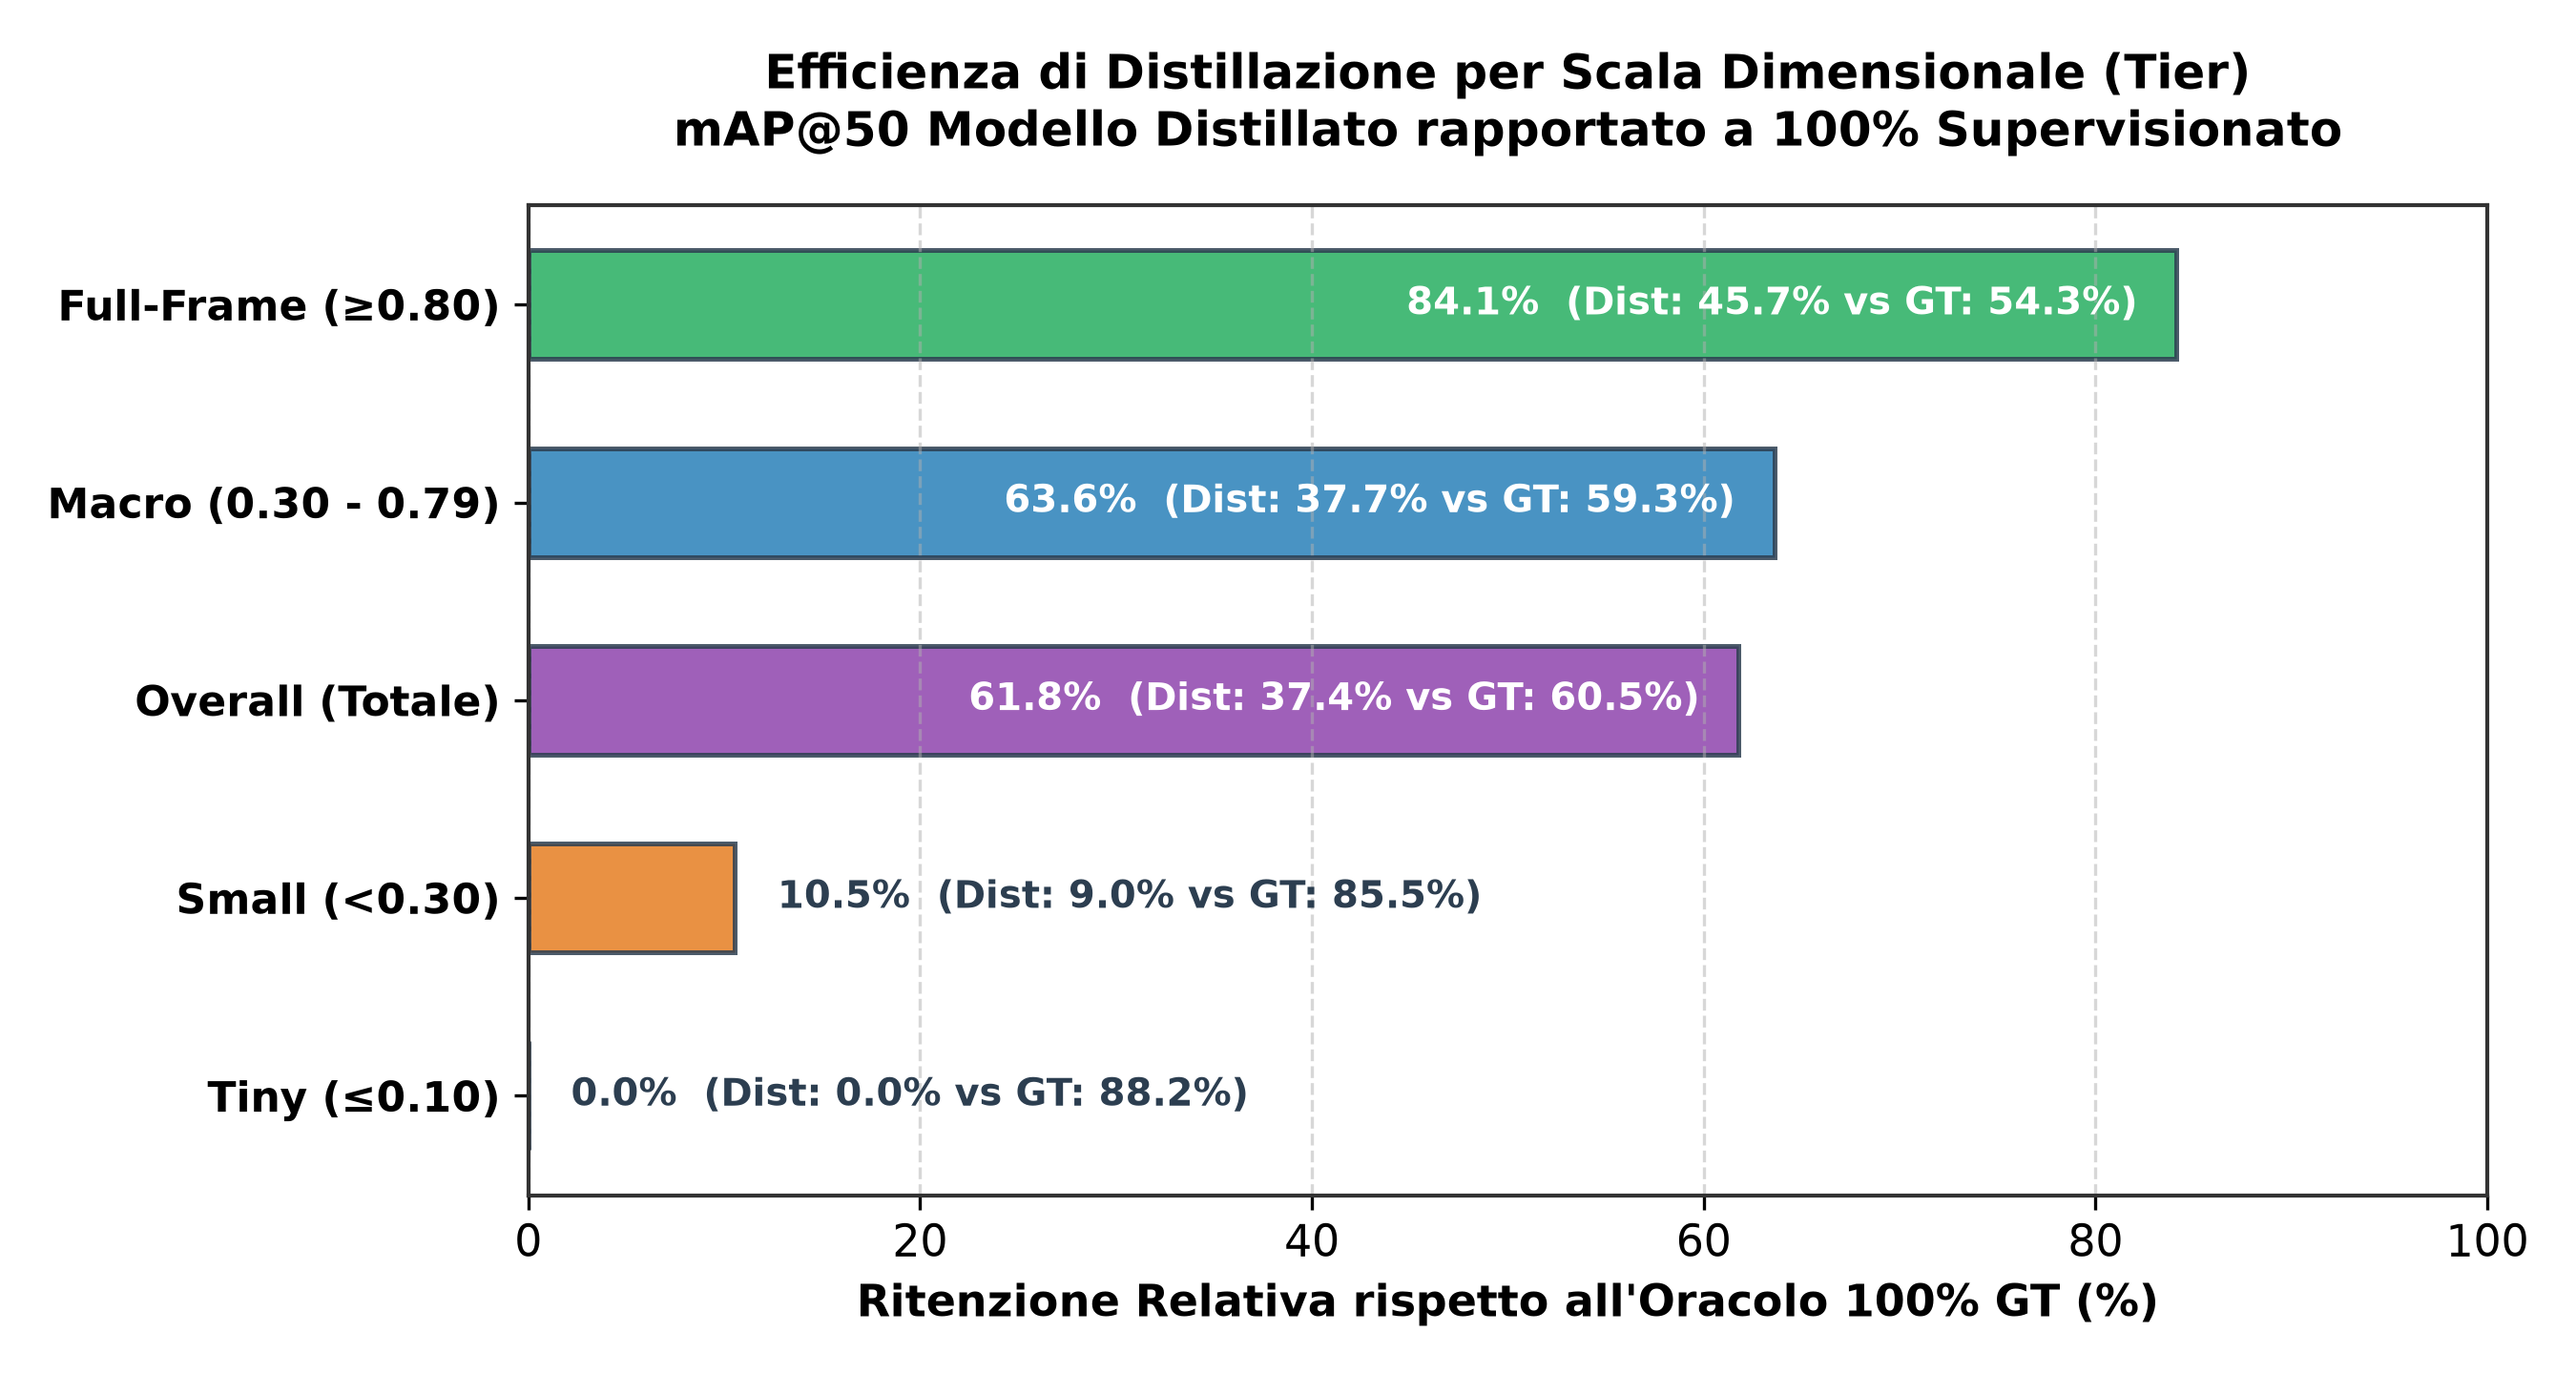
\includegraphics[width=0.52\textwidth]{figure/ritenzione_per_tier.png}
\caption{Ritenzione relativa di mAP@50 dello studente distillato (0\% GT) rispetto all'oracolo 100\% disaggregata per tier dimensionale.}
\label{fig:ritenzione_per_tier}
\end{figure}

Il riscontro più significativo sul piano applicativo riguarda il Tier Macro (26 classi, con area media compresa tra il $30\%$ e il $79\%$ del fotogramma), che raccoglie altari, portali e affreschi. In questa fascia, dove la localizzazione richiede l'effettiva stima dei confini rispetto allo sfondo, la pipeline mantiene il $63.60\%$ delle prestazioni dell'oracolo e supera la baseline supervisionata all'$1\%$ ($37.71\%$ contro $32.42\%$). Nei soggetti di dimensioni ridotte (Tier Small e Tiny) le prestazioni invece scendono bruscamente, azzerandosi sulle 4 classi del Tier Tiny.

\section{Analisi del Tier Tiny: Bias Contestuale e Attribution Leakage}
\label{sec:ris_tiny_bias}
Il mancato rilevamento sul Tier Tiny ($0.00\%$ mAP@50 sulle 4 classi \textit{Sant'Agata}, \textit{Cupola}, \textit{Santa Scolastica} e \textit{Bassorilievi Mancanti}) non dipende dalla risoluzione a griglia ($24 \times 24$ patch), ma da un problema di selezione delle feature discriminative (Figura~\ref{fig:bias_contestuale_tiny}).

\begin{figure}[!htbp]
\centering
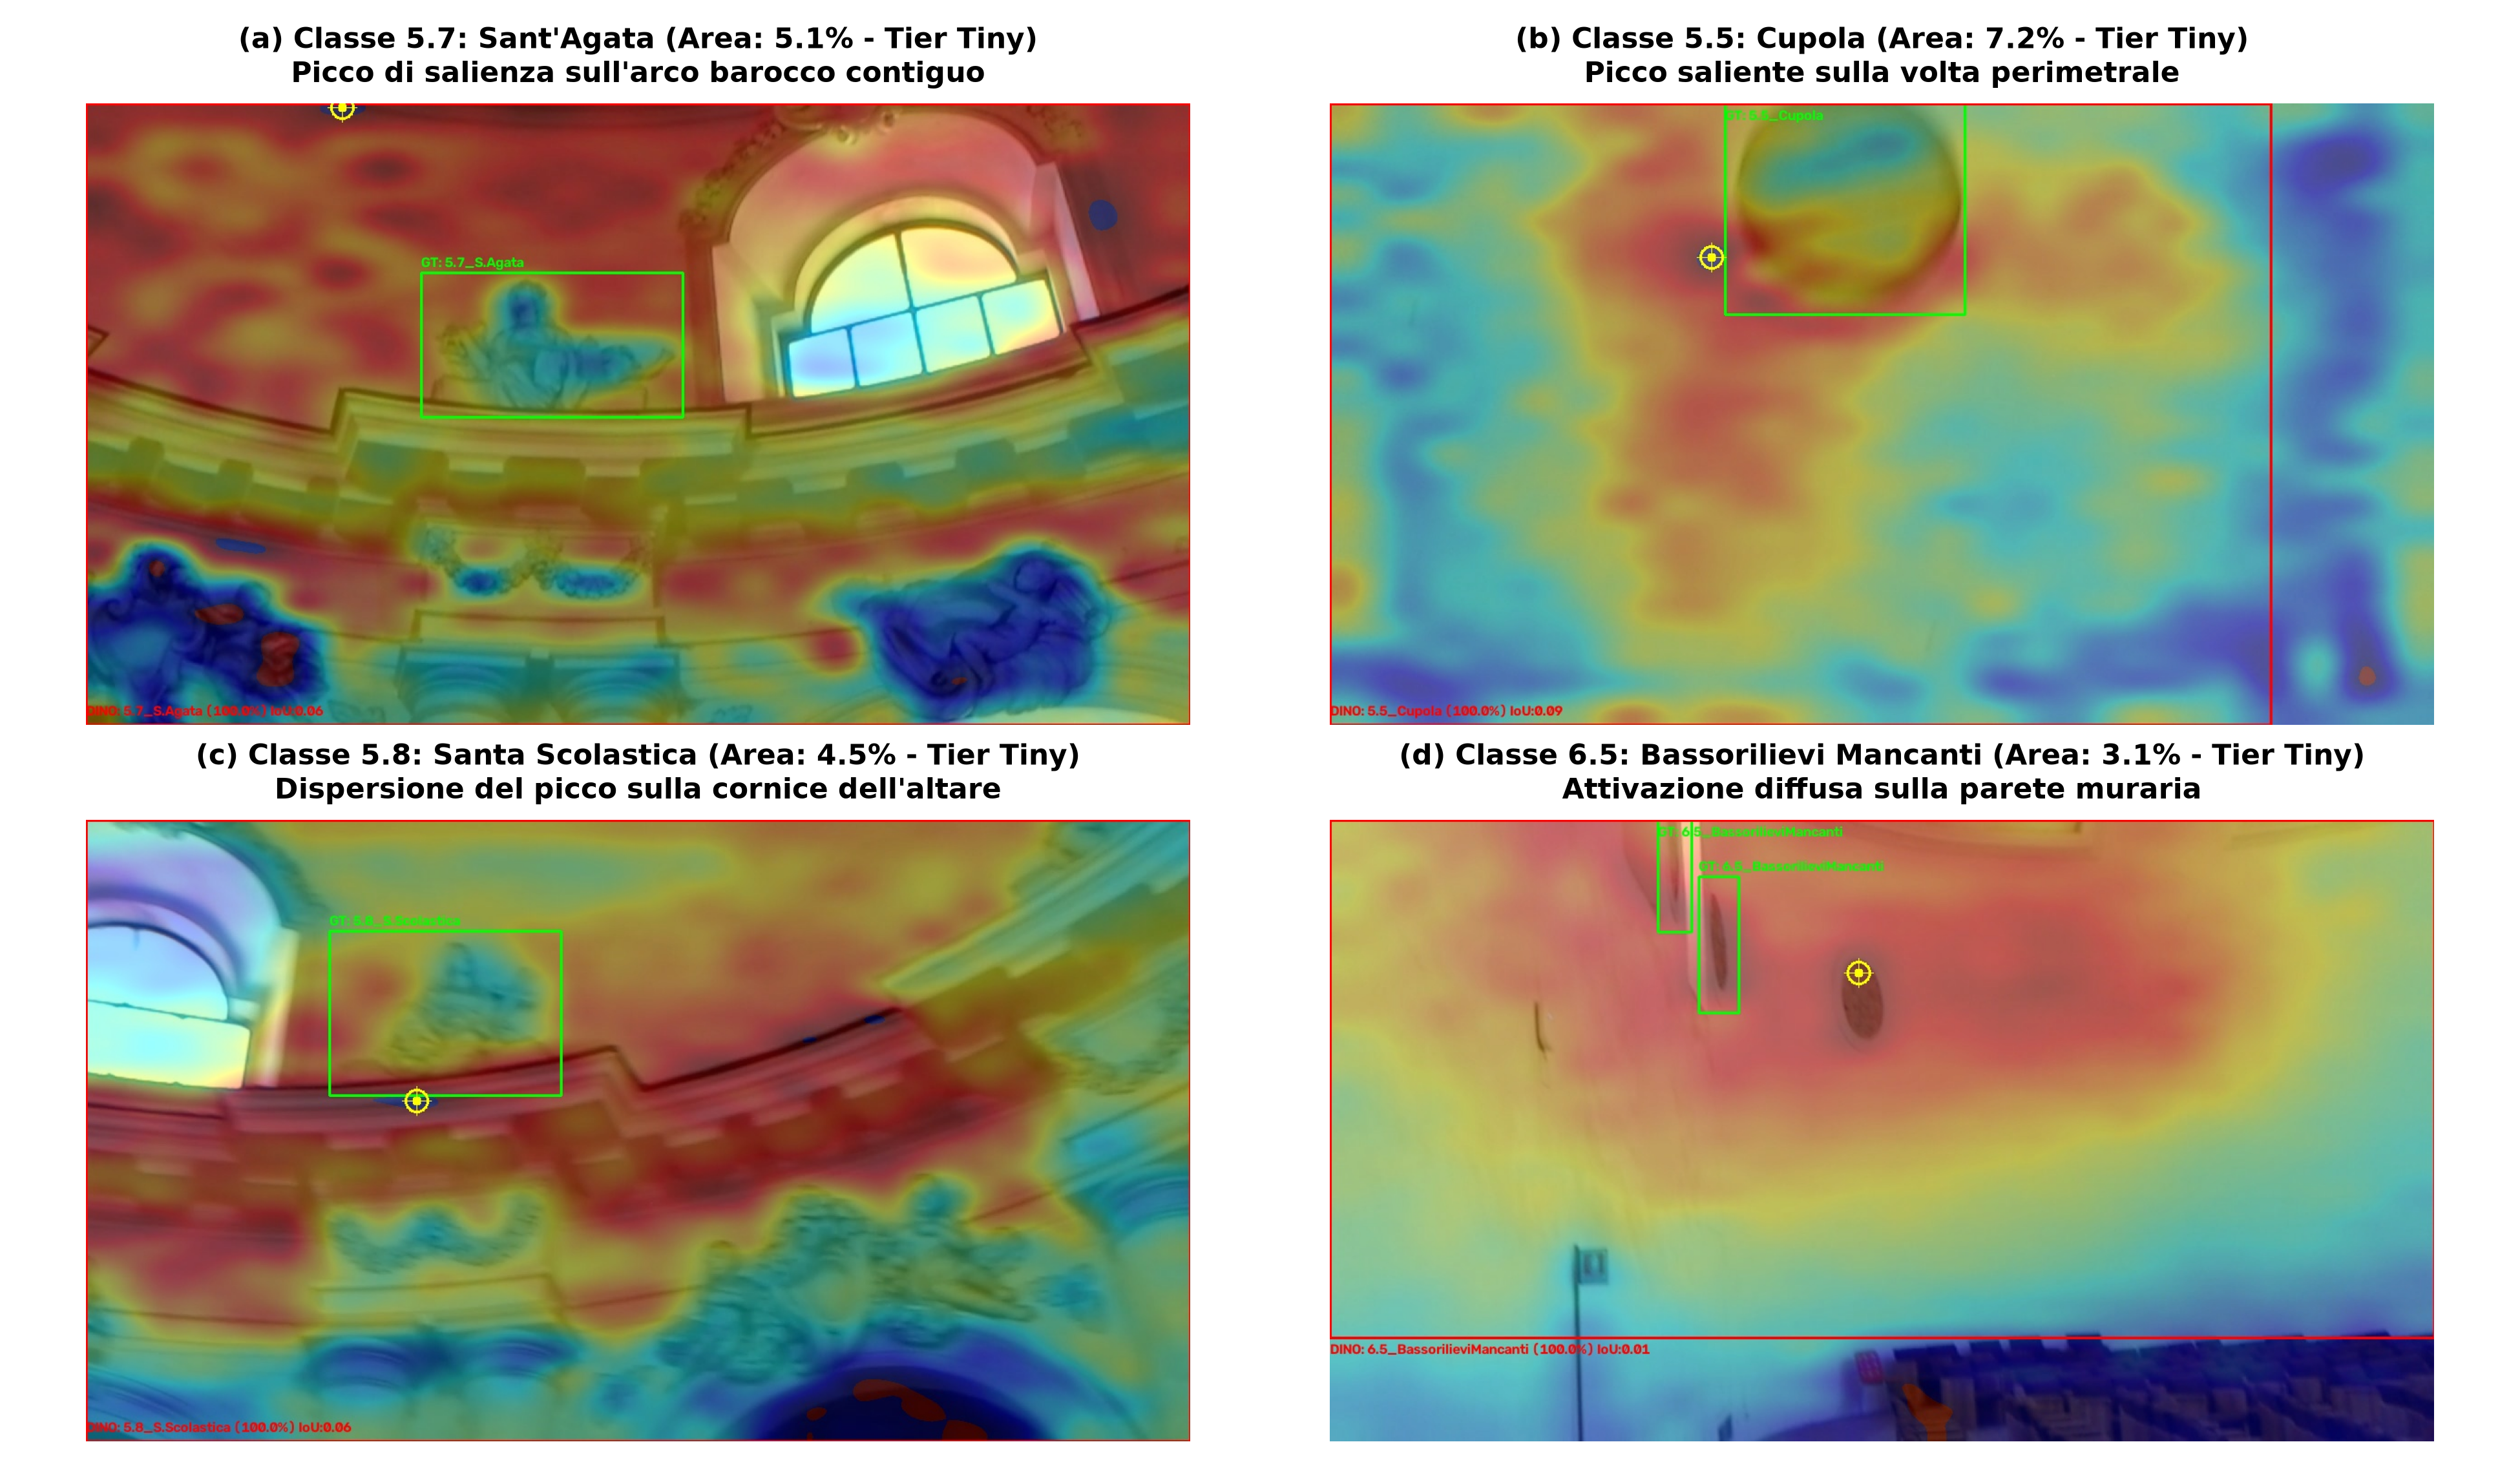
\includegraphics[width=0.82\textwidth]{figure/bias_contestuale_tiny.png}
\caption{Disallineamento discriminativo sui quattro soggetti del Tier Tiny: (a) Sant'Agata (area 5.1\%), (b) Cupola (area 7.2\%), (c) Santa Scolastica (area 4.5\%) e (d) Bassorilievi Mancanti (area 3.1\%). In tutti i casi le mappe di salienza isolano porzioni del reperto, ma il picco globale di attivazione (mirino giallo) si sposta sulla struttura architettonica contigua o sullo sfondo murario, generando uno pseudo-box errato (rosso) rispetto al Ground Truth (verde).}
\label{fig:bias_contestuale_tiny}
\end{figure}

Osservando le attivazioni locali, si nota che DINOv3 separa con chiarezza la silhouette dell'oggetto dalle pareti. Il picco massimo ($\arg\max \mathcal{H}$), tuttavia, scivola sulle strutture architettoniche limitrofe o sulle superfici contigue (l'arco per Sant'Agata, la volta per la Cupola, la cornice per Santa Scolastica, la parete muraria per i Bassorilievi Mancanti).
Questo comportamento discende dal bias contestuale insito nella supervisione d'immagine:
\begin{enumerate}
    \item La funzione di costo $\mathcal{L}_{\text{CE}}$ premia qualunque indizio visivo utile a distinguere la classe dalle altre 56 presenti nell'edificio.
    \item Un manufatto di piccole dimensioni co-occorre in modo costante con lo sfondo architettonico fisso (l'arco o la volta), che offre una superficie visiva molto più estesa e ricca di pattern.
    \item Il modello apprende una scorciatoia statistica (\textit{shortcut learning}): riconosce la scena con precisione ($94.38\%$), ma posiziona il picco di calore sull'elemento di contesto anziché sull'opera, producendo un riquadro con $\text{IoU} < 0.10$ rispetto al ground truth.
\end{enumerate}

\section{Baseline Box a Tutta Immagine e Disaccoppiamento}
\label{sec:ris_fullframe}
Nel Tier Full-Frame (copertura media del $93\%$), un riquadro fisso esteso all'intero fotogramma $[0.5, 0.5, 1.0, 1.0]$ produce per pura geometria un $\text{IoU} \approx 0.93 \gg 0.50$. In questa fascia, localizzare debolmente l'oggetto coincide nei fatti con la corretta classificazione della scena.
Nel Tier Macro, invece, il riquadro banale fallisce ($\text{IoU} \in [0.30, 0.79]$). Il raggiungimento del $37.71\%$ di mAP@50 e del $63.60\%$ di ritenzione conferma che la rete isola i contorni dell'oggetto dallo sfondo circostante.

\section{Gap di Generalizzazione dello Studente}
\label{sec:ris_distillazione_gap}
Il divario tra la validazione dello studente YOLOv8n ($96.64\%$ mAP@50 su pseudo-label) e la valutazione sul test set ($37.39\%$ su ground truth) riflette due fenomeni concorrenti: l'\textit{attribution leakage} sulle classi più piccole e il disallineamento cinematico tra le inquadrature stabili del training e le 7 sessioni video continue del test set.
